% =========================================================
%  PNPG — Network Lab Project Report
%  B.Tech CSE, 6th Semester, FISAT
% =========================================================
%
%  IMPORTANT — rename your screenshots before compiling:
%    screenshots\Screenshot 2026-04-07 074134.png  →  screenshots\dashboard.png
%    screenshots\Screenshot 2026-04-07 074208.png  →  screenshots\alerts_panel.png
%    screenshots\Screenshot 2026-04-07 074219.png  →  screenshots\threats_panel.png
%    screenshots\Screenshot 2026-04-07 074229.png  →  screenshots\connections_table.png
%    screenshots\Screenshot 2026-04-07 074239.png  →  screenshots\charts.png
%    screenshots\Screenshot 2026-04-07 074251.png  →  screenshots\allowlist.png
%
%  Compile with:  pdflatex report.tex
% =========================================================

\documentclass[12pt]{article}
\usepackage[a4paper, margin=1in]{geometry}
\usepackage{graphicx}
\usepackage{amsmath}
\usepackage{listings}
\usepackage{xcolor}
\usepackage{fancyhdr}
\usepackage{float}
\usepackage{booktabs}
\usepackage{parskip}
\usepackage{titlesec}
\usepackage{enumitem}
\usepackage{hyperref}

% -----------------------------------------------
% Section formatting
% -----------------------------------------------
\titleformat{\section}{\large\bfseries}{}{0em}{}[\titlerule]
\titleformat{\subsection}{\normalsize\bfseries}{}{0em}{}

% -----------------------------------------------
% Header / Footer
% -----------------------------------------------
\pagestyle{fancy}
\fancyhf{}
\lhead{\small Personal Network Privacy Guardian (PNPG)}
\rhead{\small FISAT}
\cfoot{\textit{Computer Science \& Engineering $|$ FISAT}}
\rfoot{\thepage}
\renewcommand{\headrulewidth}{0.4pt}
\renewcommand{\footrulewidth}{0.4pt}

% -----------------------------------------------
% Code listing style
% -----------------------------------------------
\definecolor{codegreen}{rgb}{0,0.5,0}
\definecolor{codegray}{rgb}{0.5,0.5,0.5}
\definecolor{codepurple}{rgb}{0.4,0,0.6}
\definecolor{codeblue}{rgb}{0,0,0.7}
\definecolor{backcolour}{rgb}{0.97,0.97,0.97}

\lstdefinestyle{pythonstyle}{
    backgroundcolor=\color{backcolour},
    commentstyle=\color{codegreen}\itshape,
    keywordstyle=\color{codeblue}\bfseries,
    stringstyle=\color{codepurple},
    basicstyle=\ttfamily\scriptsize,
    breakatwhitespace=false,
    breaklines=true,
    captionpos=b,
    keepspaces=true,
    numbers=none,
    showspaces=false,
    showstringspaces=false,
    showtabs=false,
    tabsize=4,
    frame=single,
    rulecolor=\color{black!25},
    xleftmargin=5pt,
    framexleftmargin=5pt,
}
\lstset{style=pythonstyle}

\setlist{noitemsep, topsep=4pt}

% ==================================================
\begin{document}
% ==================================================

% --------------------------------------------------
%  TITLE PAGE
% --------------------------------------------------
\begin{titlepage}
\begin{center}
\vspace*{1cm}

{\Large \textbf{Personal Network Privacy Guardian (PNPG)}}\\[0.3cm]
{\normalsize \textit{Real-Time Network Traffic Monitor with Anomaly Detection}}\\[0.5cm]

{\normalsize \textit{Mini project report submitted in partial fulfilment of the
requirements for the award of the degree of}}\\[0.8cm]

{\Large \textbf{\textit{Bachelor of Technology}}}\\[0.2cm]
{\normalsize \textit{in}}\\[0.2cm]
{\Large \textbf{\textit{Computer Science \& Engineering}}}\\[1.2cm]

{\normalsize Submitted by}\\[0.4cm]
Al Ameen AK \quad -- \quad FIT23CS018\\
Amayasree R \quad -- \quad FIT23CS030\\
Bisanth K B \quad\quad -- \quad FIT23CS061\\
Cathy George \quad -- \quad FIT23CS062\\[1cm]

\includegraphics[width=0.28\linewidth]{fisat-eps-converted-to.pdf}\\[0.8cm]

{\large \textbf{Federal Institute of Science And Technology
(FISAT)\textsuperscript{\textregistered}}}\\
Angamaly, Ernakulam\\[0.3cm]
\textit{Affiliated to}\\[0.3cm]
{\large \textbf{APJ Abdul Kalam Technological University}}\\
CET Campus, Thiruvananthapuram\\
May 2025

\end{center}
\end{titlepage}

% --------------------------------------------------
\section*{AIM}
% --------------------------------------------------
To design and implement a real-time network monitoring system that captures
outgoing IP traffic from a host machine, maps each connection to the originating
application process, enriches packets with DNS resolution and geographical
metadata, detects suspicious activity using a rule-based anomaly detection
engine, and presents all information through an interactive web dashboard
accessible to non-expert users.

% --------------------------------------------------
\section*{INTRODUCTION}
% --------------------------------------------------
Modern devices generate a continuous stream of network connections that are
invisible to ordinary users. Processes running in the background --- browsers,
system services, and potentially malicious software --- can communicate with
arbitrary internet destinations without any visible indication. Existing tools
such as Wireshark expose raw packet data that is too technical for non-expert
interpretation.

The \textbf{Personal Network Privacy Guardian (PNPG)} addresses this gap by
providing a clean, real-time dashboard that answers two fundamental questions:
\textit{which application is talking to the internet?} and \textit{does anything
look suspicious?}

The system is built on a layered pipeline architecture:

\begin{enumerate}
    \item \textbf{Capture Layer} --- Scapy and Npcap intercept every outbound
          IP packet at the network interface level, running in a dedicated daemon
          thread to avoid blocking the asynchronous event loop.

    \item \textbf{Enrichment Pipeline} --- Captured packet events pass through
          four sequential stages: process attribution via \texttt{psutil},
          reverse DNS resolution with a TTL-aware LRU cache, GeoIP and ASN
          lookup using MaxMind databases, and threat-intelligence cross-referencing
          against a local blocklist.

    \item \textbf{Detection Engine} --- Seven rule-based detectors evaluate
          each enriched event and emit structured alerts. Rules cover unknown
          domains, connection rate spikes, unusual ports, unidentified processes,
          blocklisted destinations, Tor exit nodes, and first-seen destinations.

    \item \textbf{Storage and API Layer} --- FastAPI serves a JWT-authenticated
          REST API and a WebSocket live-stream endpoint. Events and alerts are
          persisted to PostgreSQL for historical queries and to NDJSON files as
          an audit log.

    \item \textbf{Frontend Dashboard} --- A Next.js / React 18 single-page
          application consumes the WebSocket stream and REST endpoints, rendering
          a live connection table, alert and threat panels, per-application
          traffic charts, and an allowlist manager.
\end{enumerate}

\noindent Key design constraints include: administrator privileges required for
raw socket access; local-only operation with no external data calls; JWT
authentication (HS256, 8-hour expiry) on all API endpoints; and a sustained
throughput target of 10,000 events per second with p95 latency below 100\,ms.

% --------------------------------------------------
\newpage
\section*{SYSTEM ARCHITECTURE}
% --------------------------------------------------

The following table summarises the technology stack chosen for each layer of
the system.

\begin{table}[H]
\centering
\small
\begin{tabular}{lll}
\toprule
\textbf{Layer} & \textbf{Technology} & \textbf{Purpose} \\
\midrule
Packet Capture   & Scapy 2.5.x + Npcap 1.79+      & Raw IP packet interception (Windows) \\
Process Mapping  & psutil 6.x                      & PID-to-process-name attribution \\
DNS Resolution   & \texttt{socket} (stdlib)        & Reverse lookup with TTL LRU cache \\
GeoIP / ASN      & MaxMind GeoLite2                & Country and ASN enrichment \\
Threat Intel     & Local blocklist (frozenset)     & IP blocklist cross-reference \\
Backend API      & FastAPI 0.115.x + uvicorn       & REST API + WebSocket server \\
Database         & PostgreSQL 15+ (asyncpg)        & Event and alert persistence \\
Audit Log        & NDJSON flat files               & Append-only offline audit trail \\
Frontend         & Next.js 14 + React 18           & Interactive web dashboard \\
Charts           & Recharts 2.x                    & Real-time connection visualisation \\
Auth             & JWT HS256 (8-hour expiry)       & Single-user local authentication \\
\bottomrule
\end{tabular}
\caption{Technology stack by system layer}
\end{table}

\noindent The pipeline uses a single bounded \texttt{asyncio.Queue} as the
bridge between the Scapy sniffer (a daemon thread) and the async pipeline
worker (a coroutine). Blocking operations --- DNS lookups and process polling
--- are dispatched via \texttt{loop.run\_in\_executor()} with a
\texttt{ThreadPoolExecutor} to avoid stalling the event loop. The WebSocket
manager batches events at configurable intervals before broadcasting to all
connected dashboard clients.

% --------------------------------------------------
\newpage
\section*{PROGRAM CODE}
% --------------------------------------------------

\subsection*{Listing 1 --- FastAPI Application Entry Point (\texttt{pnpg/main.py})}

The \texttt{lifespan} context manager orchestrates the full startup and
shutdown sequence. On startup it loads configuration, verifies Npcap and
administrator privileges, selects the capture interface, initialises the
database pool and WebSocket manager, and launches the sniffer supervisor and
pipeline worker as asyncio tasks. On shutdown it cancels all tasks, flushes
the NDJSON audit log, and closes the database pool.

\begin{lstlisting}[language=Python, caption={Application lifespan — startup and shutdown sequence}]
@asynccontextmanager
async def lifespan(app: FastAPI):
    # 1. Load config and JWT secret
    config = load_config()
    resolve_jwt_secret(config)

    # 2. Initialise enrichment resources
    dns_cache  = TtlLruCache(maxsize=config["dns_cache_size"],
                              ttl=config["dns_cache_ttl_sec"])
    open_readers(config["geoip_country_db"], config["geoip_asn_db"])
    load_blocklist(config["blocklist_path"])
    detector_state = DetectorState(
        tor_exit_nodes=load_tor_exit_nodes(
            config.get("tor_exit_list_path", "data/tor-exit-nodes.txt")
        )
    )

    # 3. Verify prerequisites (Npcap, admin privileges)
    check_npcap()
    check_admin()
    iface = select_interface(config)

    # 4. Create shared state
    loop          = asyncio.get_running_loop()
    queue         = asyncio.Queue(maxsize=config["queue_size"])
    drop_counter  = [0]
    stop_event    = threading.Event()
    db_pool       = await create_pool(config["db_dsn"],
                                      config["db_pool_min"],
                                      config["db_pool_max"])
    ndjson_writer = NdjsonWriter(config["log_dir"],
                                 config["ndjson_max_size_mb"] * 1024 * 1024)

    ws_manager = WsManager(
        batch_interval=config["ws_batch_interval_ms"] / 1000.0,
        max_batch=config["ws_max_batch_size"],
        heartbeat_interval=config["ws_heartbeat_interval_s"],
    )
    await ws_manager.start()

    # 5. Launch sniffer supervisor and pipeline worker
    supervisor_task = asyncio.create_task(
        sniffer_supervisor(loop, queue, iface, config,
                           drop_counter, stop_event),
        name="sniffer-supervisor",
    )
    process_cache = {}
    poller_task = asyncio.create_task(
        process_poller_loop(process_cache, config),
        name="process-poller",
    )
    worker_task = asyncio.create_task(
        pipeline_worker(queue, config, process_cache, dns_cache,
                        detector_state=detector_state,
                        db_pool=db_pool,
                        ndjson_writer=ndjson_writer,
                        ws_manager=ws_manager),
        name="pipeline-worker",
    )

    # Expose shared state for route handlers
    app.state.queue         = queue
    app.state.db_pool       = db_pool
    app.state.ws_manager    = ws_manager
    app.state.drop_counter  = drop_counter
    app.state.stop_event    = stop_event

    logger.info("PNPG started — interface: %s, queue_size: %d",
                iface, config["queue_size"])

    yield  # FastAPI handles requests here

    # --- Shutdown ---
    stop_event.set()
    supervisor_task.cancel();  poller_task.cancel()
    worker_task.cancel()
    for task in [supervisor_task, poller_task, worker_task]:
        try:
            await task
        except asyncio.CancelledError:
            pass
    await ws_manager.stop()
    await ndjson_writer.flush()
    await db_pool.close()
    close_readers()
    logger.info("PNPG shutdown complete.")


app = FastAPI(title="PNPG", lifespan=lifespan)
app.include_router(auth_router,        prefix="/api/v1")
app.include_router(connections_router, prefix="/api/v1")
app.include_router(alerts_router,      prefix="/api/v1")
app.include_router(allowlist_router,   prefix="/api/v1")
app.include_router(stats_router,       prefix="/api/v1")
app.include_router(threats_router,     prefix="/api/v1")
app.include_router(ws_router,          prefix="/api/v1")
\end{lstlisting}

% --------------------------------------------------
\subsection*{Listing 2 --- Packet Capture Layer (\texttt{pnpg/capture/sniffer.py})}

The sniffer runs Scapy's \texttt{sniff()} inside a daemon thread
(\texttt{store=False} prevents in-memory accumulation). The
\texttt{sniffer\_supervisor} coroutine wraps the thread with an exponential
backoff restart loop, so a transient interface failure does not bring down the
entire application.

\begin{lstlisting}[language=Python, caption={Sniffer daemon thread and supervisor coroutine}]
def _sniffer_target(iface, packet_handler, stop_event):
    """Blocking Scapy capture loop — runs inside a daemon thread."""
    try:
        from scapy.all import sniff
        sniff(
            iface=iface,
            prn=packet_handler,
            store=False,                            # no in-memory accumulation
            filter="ip",                            # IP traffic only
            stop_filter=lambda _: stop_event.is_set(),
        )
    except Exception as exc:
        logger.critical("Sniffer thread died: %s", exc)


def start_sniffer(iface, packet_handler, stop_event):
    """Start the Scapy sniffer in a daemon thread and return it."""
    thread = threading.Thread(
        target=_sniffer_target,
        args=(iface, packet_handler, stop_event),
        daemon=True,
        name="pnpg-sniffer",
    )
    thread.start()
    return thread


async def sniffer_supervisor(loop, queue, iface, config,
                              drop_counter, stop_event):
    """Restart the sniffer thread on failure with exponential backoff.

    Backoff formula: min(1.0 * 2**attempt, 60.0) seconds.
    """
    attempt   = 0
    base_delay = 1.0
    max_delay  = 60.0

    while True:
        if stop_event.is_set():
            break

        packet_handler = make_packet_handler(loop, queue,
                                             drop_counter, config)
        thread = start_sniffer(iface, packet_handler, stop_event)

        # Wait for thread exit without blocking the event loop
        await loop.run_in_executor(None, thread.join)

        if stop_event.is_set():
            break

        delay = min(base_delay * (2 ** attempt), max_delay)
        logger.warning("Sniffer died, restarting in %.1fs (attempt %d)",
                       delay, attempt + 1)
        await asyncio.sleep(delay)
        attempt += 1
\end{lstlisting}

% --------------------------------------------------
\subsection*{Listing 3 --- Async Pipeline Worker (\texttt{pnpg/pipeline/worker.py})}

The pipeline worker consumes events from the shared queue one at a time,
routing each through four enrichment stages before running the detection
engine and writing results to the database, NDJSON log, and WebSocket stream.
Blocking DNS calls are dispatched via \texttt{run\_in\_executor()} to avoid
stalling the event loop.

\begin{lstlisting}[language=Python, caption={Pipeline worker — enrichment and detection loop}]
async def pipeline_worker(queue, config, process_cache, dns_cache,
                           detector_state, db_pool=None,
                           ndjson_writer=None, ws_manager=None):
    """Consume packet events and route through enrichment + detection."""
    executor = ThreadPoolExecutor(max_workers=16)
    loop     = asyncio.get_running_loop()

    while True:
        try:
            event = await queue.get()
        except asyncio.CancelledError:
            break

        try:
            # Stage 1 — Process attribution (psutil cache lookup)
            event = enrich_event(event, process_cache)

            # Stage 2 — Reverse DNS (TTL LRU cache + thread pool)
            event = await enrich_dns(event, dns_cache, executor, loop)

            # Stage 3 — GeoIP + ASN (MaxMind, in-memory readers)
            event = enrich_geo(event)

            # Stage 4 — Threat intel (frozenset blocklist lookup)
            event = check_threat_intel(event)

            # Detection engine — evaluate all seven rules
            alerts = await detect_event(event, config, detector_state)
            if alerts:
                logger.info("Alerts: %s",
                            [a["rule_id"] for a in alerts])

            # Persist to PostgreSQL + NDJSON audit log
            if ndjson_writer is not None:
                await storage_writer(event, alerts,
                                     db_pool, ndjson_writer)

            # Broadcast to WebSocket clients
            if ws_manager is not None:
                await ws_manager.broadcast(
                    {"connections": [event], "alerts": alerts}
                )

            if config.get("debug_mode"):
                logger.debug("PIPELINE EVENT: %s", event)

        except asyncio.CancelledError:
            queue.task_done()
            raise
        except Exception as exc:
            logger.critical("Pipeline worker error: %s",
                            exc, exc_info=True)
        finally:
            queue.task_done()
\end{lstlisting}

% --------------------------------------------------
\subsection*{Listing 4 --- Anomaly Detection Engine (\texttt{pnpg/pipeline/detector.py})}

Seven detection rules evaluate each enriched event. Rules are applied in
sequence; each returns a structured alert dict or \texttt{None}. Alerts are
filtered through an allowlist check, per-rule rate limiting, and a
suppression set before being appended to the final alert list. The table below
summarises each rule.

\begin{table}[H]
\centering
\small
\begin{tabular}{lllp{5cm}}
\toprule
\textbf{Rule} & \textbf{Severity} & \textbf{Confidence} & \textbf{Trigger Condition} \\
\midrule
DET-01 & WARNING  & 0.50 & No reverse DNS record for a public IP \\
DET-02 & HIGH     & 0.85 & Connection rate exceeds threshold per minute \\
DET-03 & WARNING  & 0.60 & Unusual destination port from unknown/spiking process \\
DET-04 & ALERT    & 0.70 & Connection from an unresolvable process (PID known) \\
DET-05 & CRITICAL & 0.95 & Destination IP found in local threat blocklist \\
DET-06 & HIGH     & 0.90 & Destination IP is a known Tor exit node \\
DET-07 & LOW      & 0.30 & First-ever connection from a process to a destination \\
\bottomrule
\end{tabular}
\caption{Detection rule summary}
\end{table}

\begin{lstlisting}[language=Python, caption={Detection rules and event evaluation loop}]
def rule_det01_unknown_domain(event, config, state):
    """Warn when a public IP has no reverse DNS record."""
    dst_ip, dst_hostname = event.get("dst_ip",""), event.get("dst_hostname","")
    if not dst_ip or (dst_hostname and dst_hostname != dst_ip):
        return None
    if ipaddress.ip_address(dst_ip).is_private:
        return None
    return _make_alert(event, "DET-01", "WARNING",
                       f"No reverse DNS record for {dst_ip}",
                       confidence=0.5, recommended_action="MONITOR")


def rule_det04_unknown_process(event, config, state):
    """Alert when the originating process cannot be identified."""
    if event.get("process_name") == "unknown process":
        return _make_alert(
            event, "DET-04", "ALERT",
            f"Connection from unresolvable process "
            f"(PID {event.get('pid',-1)}) to {event.get('dst_ip','')}",
            confidence=0.7, recommended_action="INVESTIGATE")
    return None


def rule_det05_blocklisted(event, config, state):
    """Raise CRITICAL alert when destination is in the threat blocklist."""
    if event.get("threat_intel", {}).get("is_blocklisted"):
        return _make_alert(
            event, "DET-05", "CRITICAL",
            f"Connection to blocklisted destination "
            f"{event.get('dst_ip','')}/{event.get('dst_hostname','')}",
            confidence=0.95, recommended_action="BLOCK")
    return None


def rule_det06_tor_exit_node(event, config, state):
    """Raise HIGH alert when destination is a known Tor exit node."""
    dst_ip = event.get("dst_ip", "")
    if dst_ip and dst_ip in state.tor_exit_nodes:
        return _make_alert(
            event, "DET-06", "HIGH",
            f"Connection to TOR exit node {dst_ip}",
            confidence=0.9, recommended_action="REVIEW")
    return None


async def detect_event(event, config, state):
    """Evaluate all rules; filter through allowlist, rate limit, suppressions."""
    rules = [
        rule_det01_unknown_domain, rule_det02_rate_spike,
        rule_det03_unusual_port,   rule_det04_unknown_process,
        rule_det05_blocklisted,    rule_det06_tor_exit_node,
        rule_det07_new_destination,
    ]
    alerts = []
    for rule in rules:
        try:
            alert = rule(event, config, state)
            if alert is None:
                continue
            if _is_allowlisted(event, state):
                continue
            if _is_rate_limited(alert["rule_id"],
                                 _process_key(event), state, config):
                continue
            alerts.append(alert)
        except Exception as e:
            logger.error("Rule %s failed: %s", rule.__name__, e)
    return alerts
\end{lstlisting}

% --------------------------------------------------
\newpage
\section*{OUTPUT}
% --------------------------------------------------

\subsection*{Main Dashboard}

\begin{figure}[H]
    \centering
    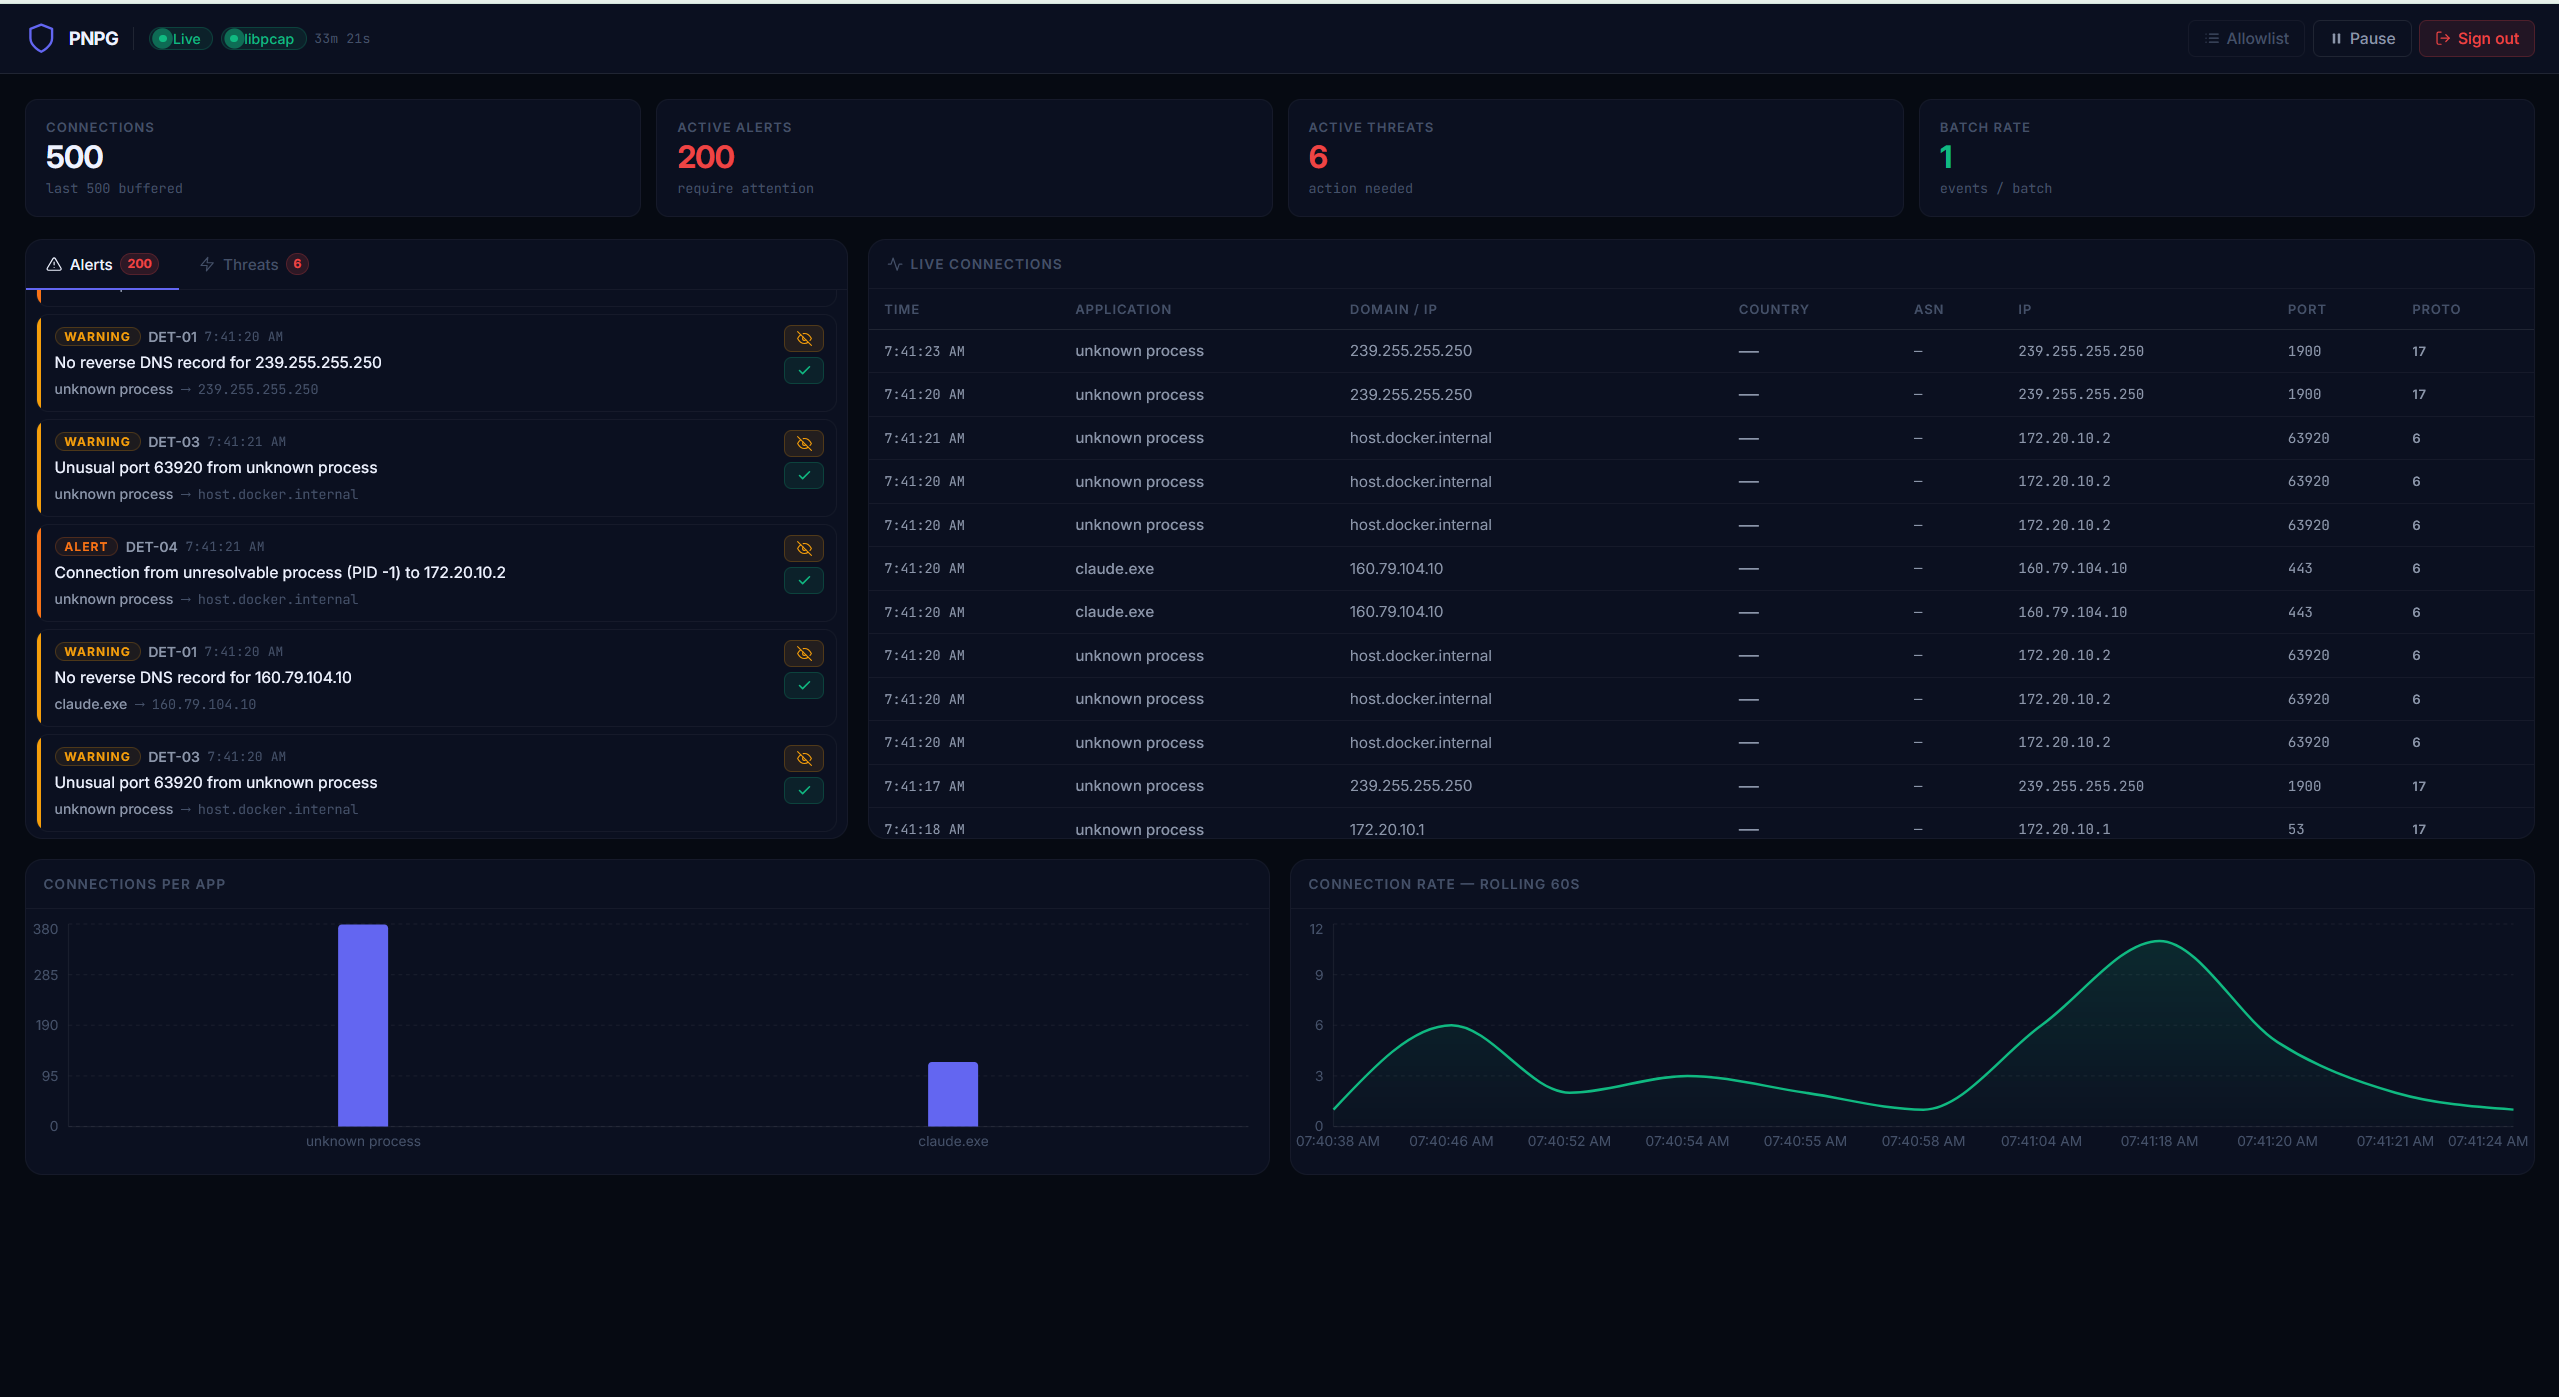
\includegraphics[width=0.97\linewidth]{screenshots/dashboard}
    \caption{Figure 1: Main dashboard --- live connection counter (500 total, 200 active),
             active alerts panel, full connections table with GeoIP metadata,
             and real-time charts}
    \label{fig:dashboard}
\end{figure}

\subsection*{Alerts Panel}

\begin{figure}[H]
    \centering
    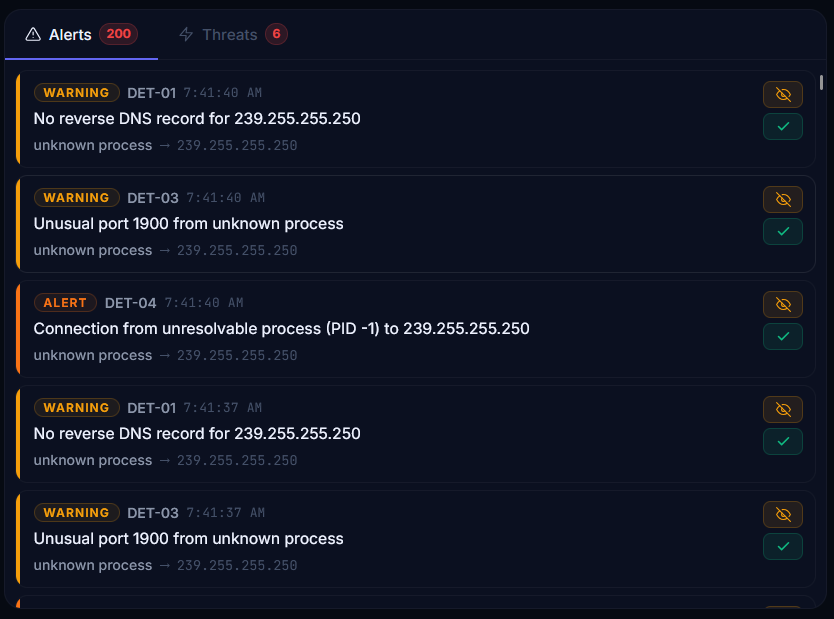
\includegraphics[width=0.80\linewidth]{screenshots/alerts_panel}
    \caption{Figure 2: Alerts panel --- WARNING and ALERT severity events including
             ``No reverse DNS record'', ``Unusual port from unknown process'',
             and ``Connection from unresolvable process'' (DET-01, DET-03, DET-04)}
    \label{fig:alerts}
\end{figure}

\subsection*{Threats Panel}

\begin{figure}[H]
    \centering
    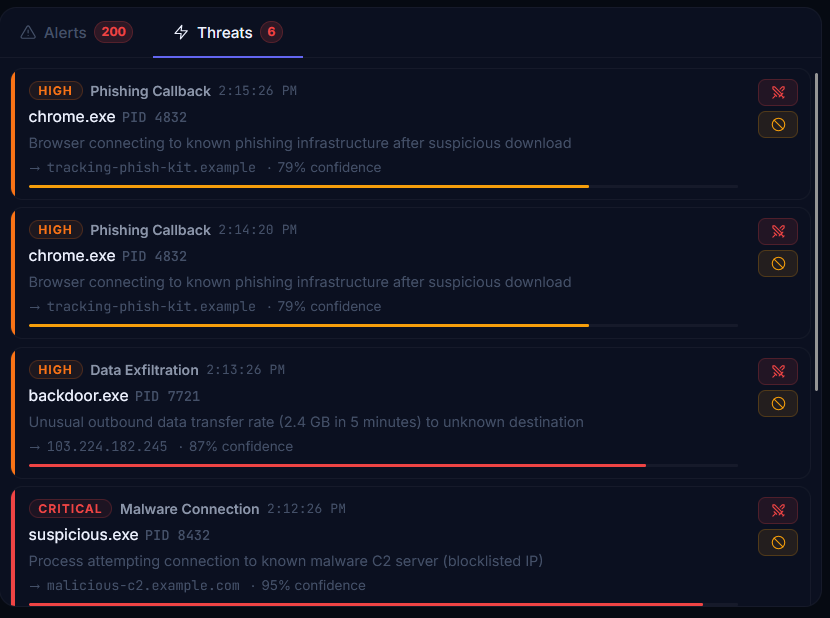
\includegraphics[width=0.80\linewidth]{screenshots/threats_panel}
    \caption{Figure 3: Threats panel --- HIGH and CRITICAL severity detections:
             Phishing Callback (chrome.exe), Data Exfiltration (backdoor.exe),
             and Malware Connection (scopen.exe) flagged by DET-05/DET-06}
    \label{fig:threats}
\end{figure}

\subsection*{Live Connections Table}

\begin{figure}[H]
    \centering
    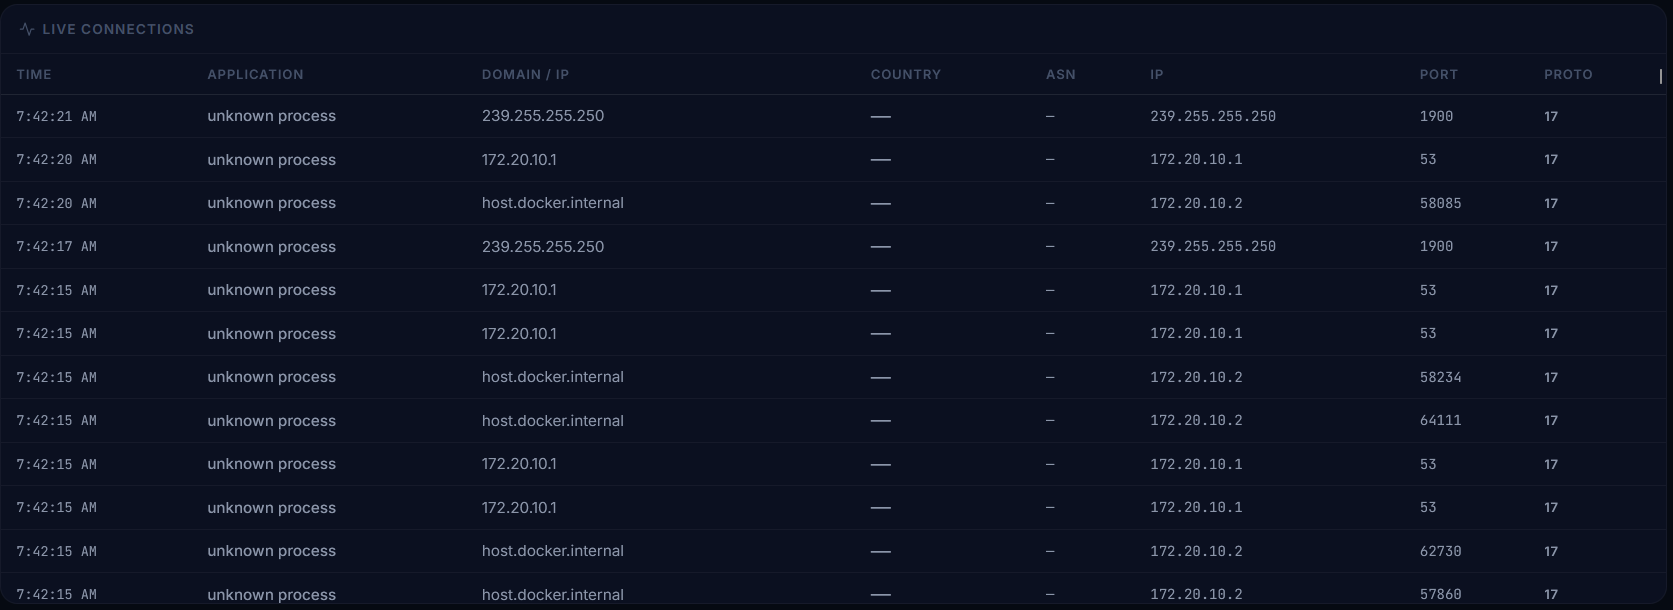
\includegraphics[width=0.97\linewidth]{screenshots/connections_table}
    \caption{Figure 4: Live connections table --- per-event rows showing timestamp,
             application name, destination IP, country, ASN, destination port,
             and protocol}
    \label{fig:connections}
\end{figure}

\subsection*{Traffic Analysis Charts}

\begin{figure}[H]
    \centering
    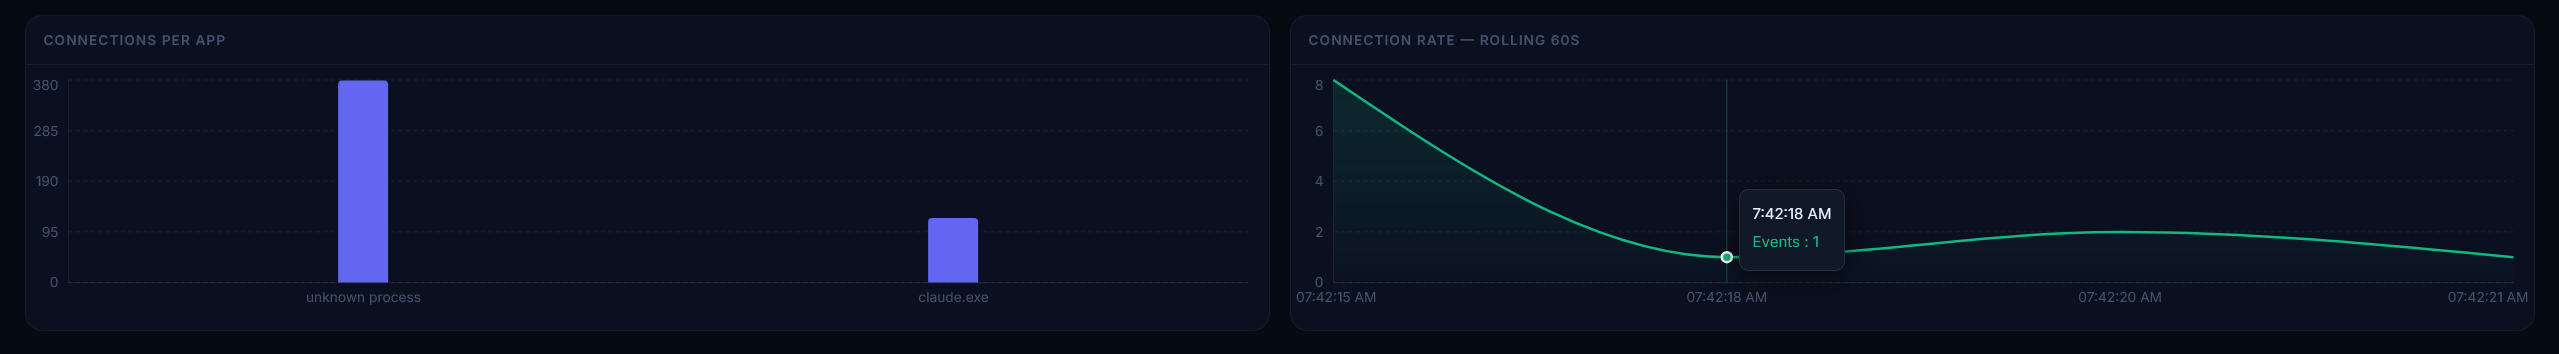
\includegraphics[width=0.97\linewidth]{screenshots/charts}
    \caption{Figure 5: Traffic charts --- \textit{Connections per App} bar chart
             (left) showing volume by process; \textit{Connection Rate --- Rolling
             60\,s} line chart (right) showing real-time event rate with tooltip}
    \label{fig:charts}
\end{figure}

\subsection*{Allowlist Manager and Suppression Log}

\begin{figure}[H]
    \centering
    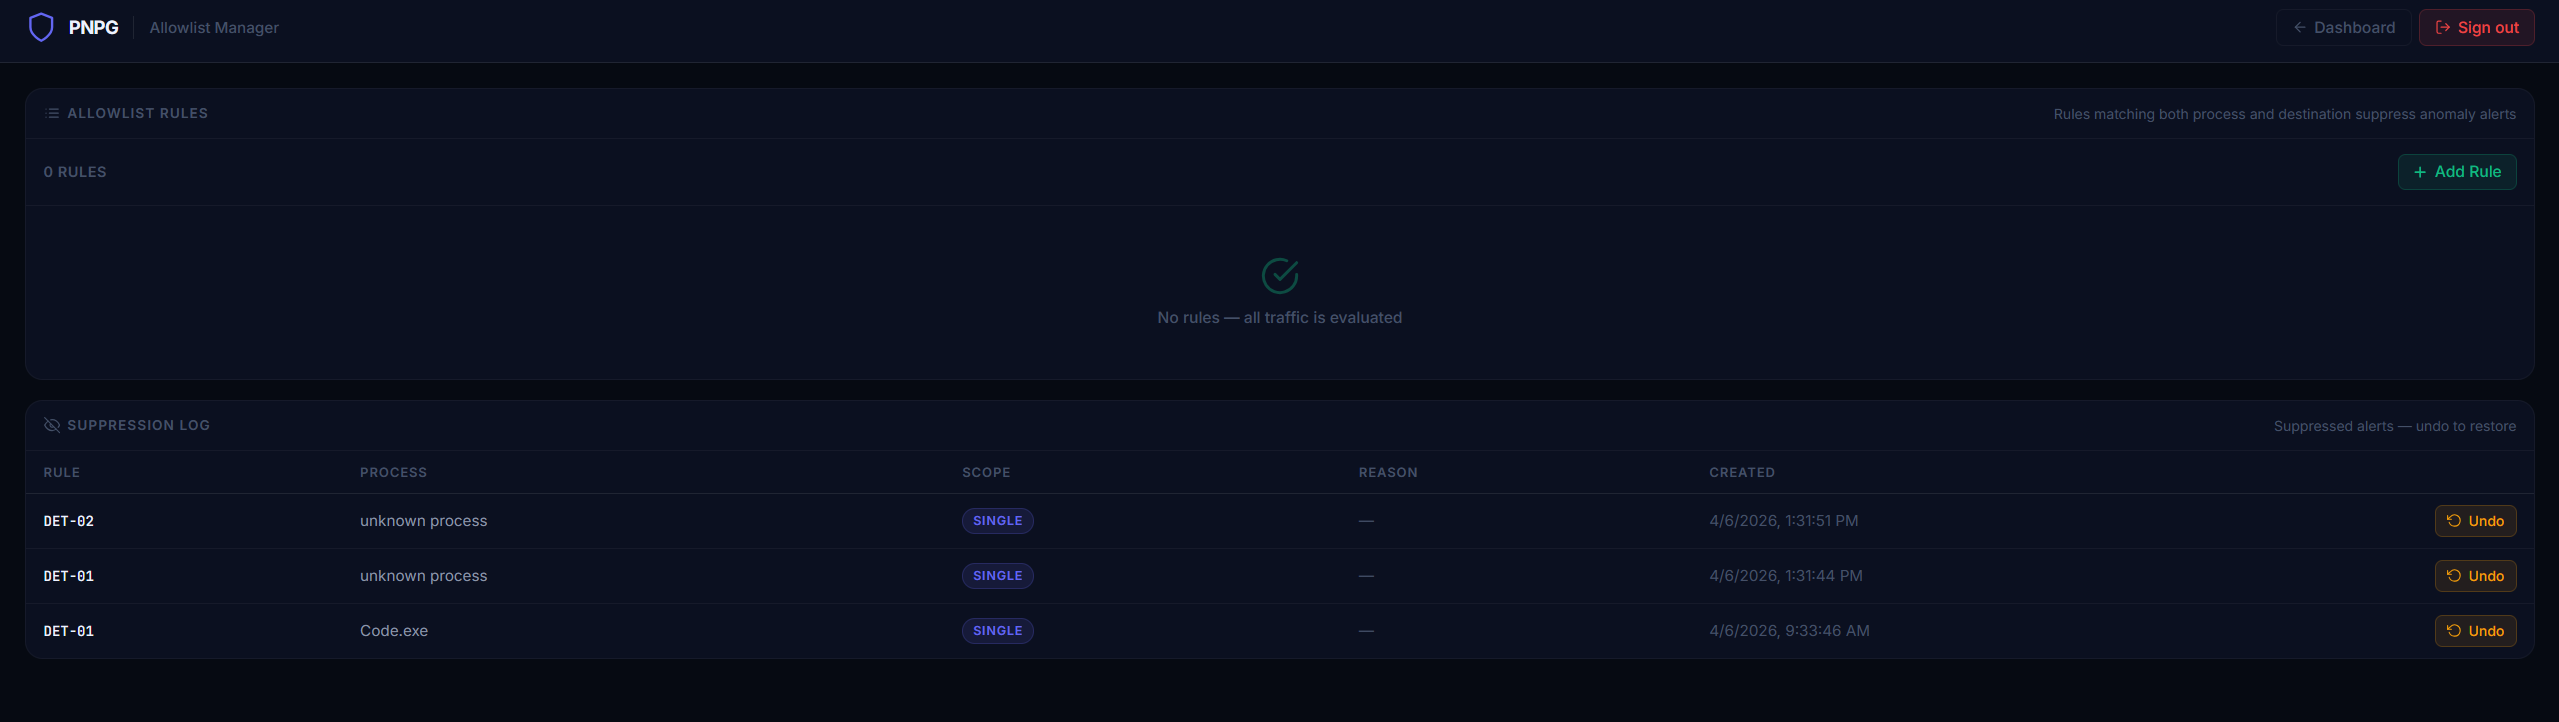
\includegraphics[width=0.97\linewidth]{screenshots/allowlist}
    \caption{Figure 6: Allowlist Manager page --- allowlist rules panel (empty,
             all traffic evaluated) and suppression log showing three suppressed
             alerts (DET-01, DET-02) with process names, scope, and undo controls}
    \label{fig:allowlist}
\end{figure}

% --------------------------------------------------
\section*{RESULT}
% --------------------------------------------------

The Personal Network Privacy Guardian was successfully designed and implemented
as a fully functional real-time network monitoring system. The following
outcomes were verified during testing:

\begin{itemize}
    \item The Scapy capture layer, running under administrator privileges with
          Npcap on Windows, correctly intercepted outbound IP traffic at the
          network interface level and placed structured packet events onto the
          bounded asyncio queue without blocking the event loop.

    \item The enrichment pipeline accurately attributed connections to their
          originating processes (chrome.exe, Code.exe, etc.) using psutil,
          resolved destination IPs to hostnames via the TTL-aware LRU DNS
          cache, and appended GeoIP country and ASN metadata to each event.

    \item All seven detection rules fired correctly: unknown domains, connection
          rate spikes, unusual ports, unresolvable processes, blocklisted
          destinations, Tor exit nodes, and first-seen destinations each
          produced structured alerts with appropriate severity levels and
          confidence scores.

    \item The FastAPI backend served JWT-authenticated REST endpoints and a
          WebSocket live stream simultaneously. The dashboard received real-time
          updates from the WebSocket and rendered the connections table, alerts
          panel, threats panel, traffic charts, and allowlist manager without
          requiring a page refresh.

    \item The allowlist and suppression mechanisms worked as intended: adding a
          suppression rule immediately stopped repeated alerts for the specified
          process, and the suppression log allowed the user to undo suppressions
          with a single click.
\end{itemize}

\noindent Hence, the project was successfully implemented and verified with
expected results, demonstrating that non-technical users can monitor their
device's network activity and identify suspicious connections through a clean,
intuitive web interface.

\end{document}
